\subchapter{Kernel optimizations}{Measure kernel boot components and
optimize the kernel boot time}

\section{Measuring}

We are going to use the kernel \code{initcall_debug} functionality.

The first thing we need to do is to recompile the kernel to make sure 
it has the right options.

So, let's get the kernel sources for our system. A source archive
is available on your USB disk. We will need 
them to recompile our kernel in a few minutes anyway.

Plug-in your USB disk and type the below commands:

\begin{verbatim}
cd /opt/felabs/boottime/kernel
cp /media/BootTime/downloads/linux-3.6.9-at91.tar.xz .
tar Jxf linux-3.6.9-at91.tar.xz
source env.sh
cd linux-3.6.9-at91
make sama5d3_defconfig
make xconfig
\end{verbatim}

Here are the contents of the \code{env.sh} file:

\begin{verbatim}
export ARCH=arm
export CROSS_COMPILE=arm-buildroot-linux-uclibcgnueabi-
export PATH=$PATH:/opt/felabs/boottime/buildroot/buildroot-at91/output/host/usr/bin/
\end{verbatim}

Now configure the kernel with the below settings:
\begin{itemize}
\item \code{CONFIG_LOG_BUF=16}. That's the size of the
      kernel ring buffer. If we keep the default size (\code{14}),
      the earliest kernel messages are overwritten by the
      latest ones.
\item Make sure that \code{CONFIG_PRINTK_TIME} is enabled
      (it should already be)
\end{itemize}

Save your configuration. We are ready to compile our kernel:
\begin{verbatim}
make -j 8 uImage 
\end{verbatim}

Keep a backup copy of your original kernel image, and copy the new one:
\footnote{So far, we are lucky to have a kernel with most drivers
compiled inside the kernel. If we had important drivers compiled 
as modules, we would need to compile the kernel with Buildroot, 
to put the updated modules in the root filesystem. We are also lucky
not to have to update the Device Tree Binary, as we are using
the same kernel sources as the demo.}

\begin{verbatim}
cd ../../flashing/sama5d3xek-demo
cp uImage uImage.orig
cp ../../kernel/linux-3.6.9-at91/arch/arm/boot/uImage .
\end{verbatim}

Reflash your system and make it boots in the same way as before. 

Now, let's enable \code{initcall_debug}. Reboot your board and press
a key to stop the U-boot countdown.

In the U-boot command line, add settings to the kernel command line
\footnote{Don't save these settings with \code{saveenv}. We
will just need them once.}
and boot your system:
\begin{verbatim}
setenv bootargs ${bootargs} initcall_debug printk.time=1
boot
\end{verbatim}

Once booted, you can store the debug information in a file:

\begin{verbatim}
dmesg > initcall_debug.log
\end{verbatim}

Copy this file to the USB disk.

Let's use the kernel script to generate a nice boot graph
from this debug information:

\begin{verbatim}
cd /opt/felabs/boottime/kernel
cp /media/BootTime/initcall_debug.log .
perl linux-3.6.9-at91/scripts/bootgraph.pl initcall_debug.log > boot.svg
\end{verbatim}

You can view the boot graph with the \code{inkscape} vector graphics
editor:

\begin{verbatim}
sudo apt-get install inkscape
inkscape boot.svg 
\end{verbatim}

\begin{center}
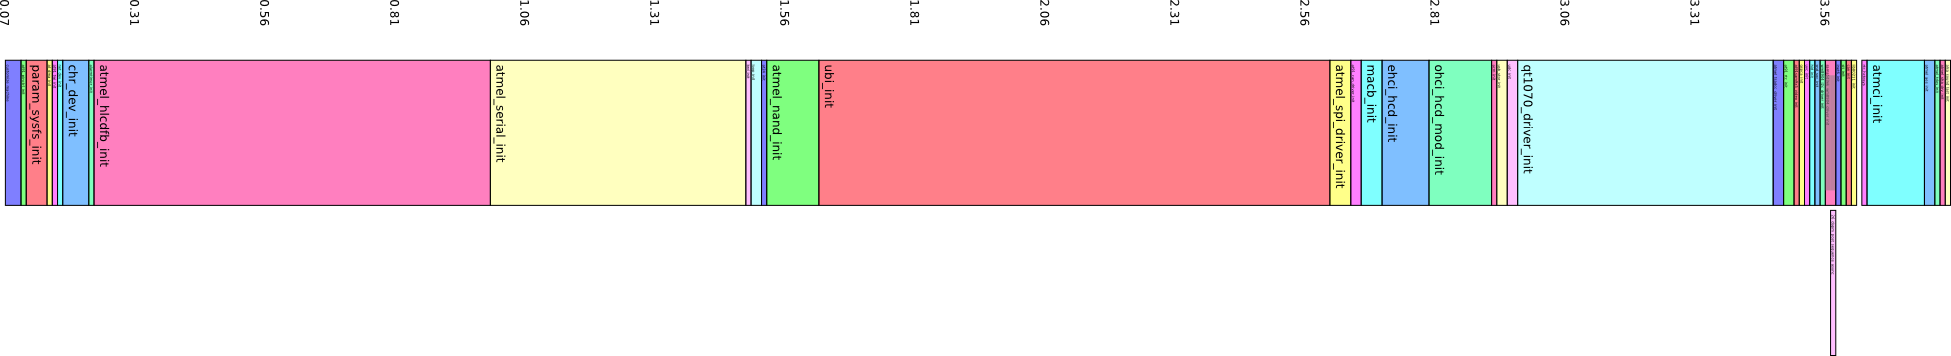
\includegraphics[width=\textwidth]{labs/boottime-kernel/boot.png}
\end{center}

Now review the longuest initcalls in detail. Each label is the name of 
a function in the kernel sources. Try to find out in which source file
each function is defined.
\footnote{You can do it with utilities such as \code{cscope}, which your
instructor will be happy to demonstrate, or through our on-line service
to explore the Linux kernel sources:
\url{http://lxr.free-electrons.com}}, and what each driver corresponds
to.

Then, you can look the source code and try look for obvious causes which
would explain the very long execution time: delay loops (look for
\code{delay}, parameters which can reduce probe time but are not used,
etc).

Before going on, reboot your board through \code{grabserial} to measure
the total boot time. The kernel rebuild could have modified it a little
bit (in case the Atmel people preparing the demo didn't use exactly the same toolchain
or kernel options as we do). Write down your result at the end of this
chapter.

\section{Reordering and postponing functionality}

The boot graph revealed drivers which could be compiled as modules 
and loaded later.  Let's compile such drivers that you found as modules
and install the corresponding modules in the root filesystem. 

Because of this requirement, we now need to compile the kernel with
Buildroot. 

First let's prepare a kernel configuration in which the selected
drivers are now compiled as modules:

\begin{verbatim}
cd /opt/felabs/boottime/kernel/linux-3.6.9-at91/
make xconfig
\end{verbatim}

For each driver, you have to look for the parameter which enables it.
If the parameter name is not trivial to find in the kernel configuration
interface, already knowing the source file implementing 
the function in the boot chart, you can look at 
the \code{Makefile} file in the same directory, and find which 
parameter is used to compile the source file in a conditional way.

Once you are done converting static drivers into modules,
copy your configuration file:

\begin{verbatim}
cp .config ../config-3.6.9-at91-with-modules
\end{verbatim}

Now go back to the Buildroot directory:

\begin{verbatim}
cd ../../buildroot/buildroot-at91
make menuconfig
\end{verbatim}

Go to the \code{Kernel} menu, and enable \code{Linux Kernel}. Now fill
the kernel related settings:

\begin{itemize}
\item \code{Kernel version}: \code{Custom tarball}
\item \code{URL of custom kernel tarball}:
      \code{http://free-electrons.com/labs/boottime/downloads/linux-3.6.9-at91.tar.xz}
\item \code{Kernel configuration}: \code{Using a custom config file}
\item \code{Configuration file path}:
      \code{/opt/felabs/boottime/kernel/config-3.6.9-at91-with-modules}
\item Enable \code{Device tree support}
\item \code{Device tree source}: \code{Use a device tree present in the kernel}
\item \code{Device Tree Source file names}: \code{sama5d34ek}
\end{itemize}

To save download time, put the Linux sources in the Buildroot download
directory. Then run Buildroot:

\begin{verbatim}
cp ../../kernel/linux-3.6.9-at91.tar.xz dl/
\end{verbatim}

Check that your modules have been added to the root filesystem:

\begin{verbatim}
find output/target -name *.ko
\end{verbatim}

The last thing to do is to load the necessary modules in a manual way 
\footnote{Oops, we don't have \code{udev} any more, and it would have
done it for us. However, manually loading modules is no big deal, and a 
simpler solution for hotplug events can still be put in place anyway.}
from the \code{/etc/init.d/rcS} file, before starting the services (SSH
will need the network driver to be loaded, for example).

Modify the \code{board/atmel/sama5d3ek_demo/rcS} file to run the
\code{modprobe} command for each of the modules before starting the
services (example: \code{modprobe macb}).

Rerun Buildroot. Before reflashing your device, this time do not only
copy \code{output/images/rootfs.ubi} but also
\code{output/images/uImage}! Reflash your device, measure the new boot time
and write it down at the end of this chapter.

\section{Removing unnecessary functionality}

The boot graph that we generated doesn't show any obvious kernel
driver that would consume a significant amount of time and could be
taken away because it is completely useless.

Of course, there will be kernel features that we will be able to remove,
in order to reduce the kernel size and make the kernel faster to load 
in the bootloader. However, this shouldn't have much impact on the
kernel's execution time. 

There's one thing we can remove though, and didn't appear on the boot
graph: we can disable console output. Writing messages on the serial
line can be very slow, especially as the serial line has a slow
bandwidth.

You can do this by adding the \code{quiet} parameter to the kernel
command line. Since we reflash the device frequently, let's store
the new setting in the flashing script.

Look for the \code{bootargs} setting in the
\code{sama5d3x_demo_linux_nandflash.tcl} file and add the \code{quiet}
parameter.

Reflash your device, measure boot time, and write in down in the summary
table.

There is another thing that is unnecessary too: the calibration of the
delay loop, as explained in the lectures. Read the \code{lpj} value from
a previous boot log, and pass this value on the kernel command line.

Measure the new boot time and write your result in the summary table.

\section{Optimizing necessary functionality}

The boot graph revealed the existence of drivers with initcalls taking a
long time to execute. It would
be worth spending time analysing their code, looking for opportunities to
reduce the initialization time taken by these drivers.

However, such investigation work could take days, unless you find
obvious issues (such as big delay loops).

\section{Results}

Fill the below table with the results from your experiments:

\begin{tabular}{| p{6cm} | c | r |}
  \hline
  Technique & Total time stamp & Difference with previous experiment \\
  \hline
  \hline
  Original time & & N/A \\
  \hline
  Postpone functionality (drivers compiled as modules) & & \\
  \hline
  Remove unnecessary functionality (\code{quiet} option) & & \\
  \hline
  Remove unnecessary functionality (skip delay loop calibration) & & \\
  \hline
  \hline
  \multicolumn{2}{| c |}{Total gain} & \\
  \hline
\end{tabular}

